Consider a family of axis-aligned ellipses $\E_t$, $0{\leq}t{\leq}\pi/3$ centered at $O_t=[0,-\sin{t}]$ with semi-axes $a,b$ given by:

\[a=\frac{\sqrt{2\,\cos{t} -1}}{2},\;\;\;b=\frac{\sqrt{(2\cos t -1)(1-\cos{t}) }}{\sqrt{2}}\]

\noindent Referring to Figure~\ref{fig:cage}(left):

\begin{remark}
The eccentricity of $\E_t$ is given by $\varepsilon_t= \sqrt{2\cos{t}-1}$. The foci $f_{1,t}$ and $f_{2,t}$ lie each on distinct unit-radius circulars arc centered on $\Cm_1,\Cm_2=[0,\mp{1/2}]$, respectively. Namely:

\[ f_{1,t},f_{2,t}=\left[\cos{t}\pm\frac{1}{2},-\sin{t}\right] \]
\label{rem:foci}
\end{remark}


 
\begin{theorem}[Continuous]
There is a continuous family of Brocard porisms $\B_t=(\Gamma_t,\E_t)$ whose 1d family of triangles:

\begin{itemize}
\item is inscribed in circle $\Gamma_t$ centered on $X_{3,t}$ with radius $R_t$ given by:
     \[ X_{3,t}=\left[0,\frac{\sin t}{2(\cos t  -1)}\right],\;\;\;R_t=\sqrt{\frac { 2\,\cos t -1}{2(1-\cos t )}} \]
\item circumscribes $\E_t$, its Brocard inellipse (i.e., its Brocard points $\Omega_{1,t},\Omega_{2,t}$ are $f_{1,t}$, $f_{2,t})$ 
\item Has fixed isodynamic points $X_{15,16}$ at $[0,\mp\sqrt{3}/2]$
\item Has fixed Brocard angle $\omega_t = t/2$% \cot^{-1}\left[\frac {\cos t +1}{\sin t }\right]$
\item Has Brocard circle $\K_t$ centered on $X_{182,t}=
[0, \frac{\cos t-2}{2\sin t}]$ with radius $\rho_t=
\frac{2\cos t-1}{ 2\sin t}$
\end{itemize}
\label{thm:continuous_iso}
\end{theorem}

\begin{figure}
    \centering
    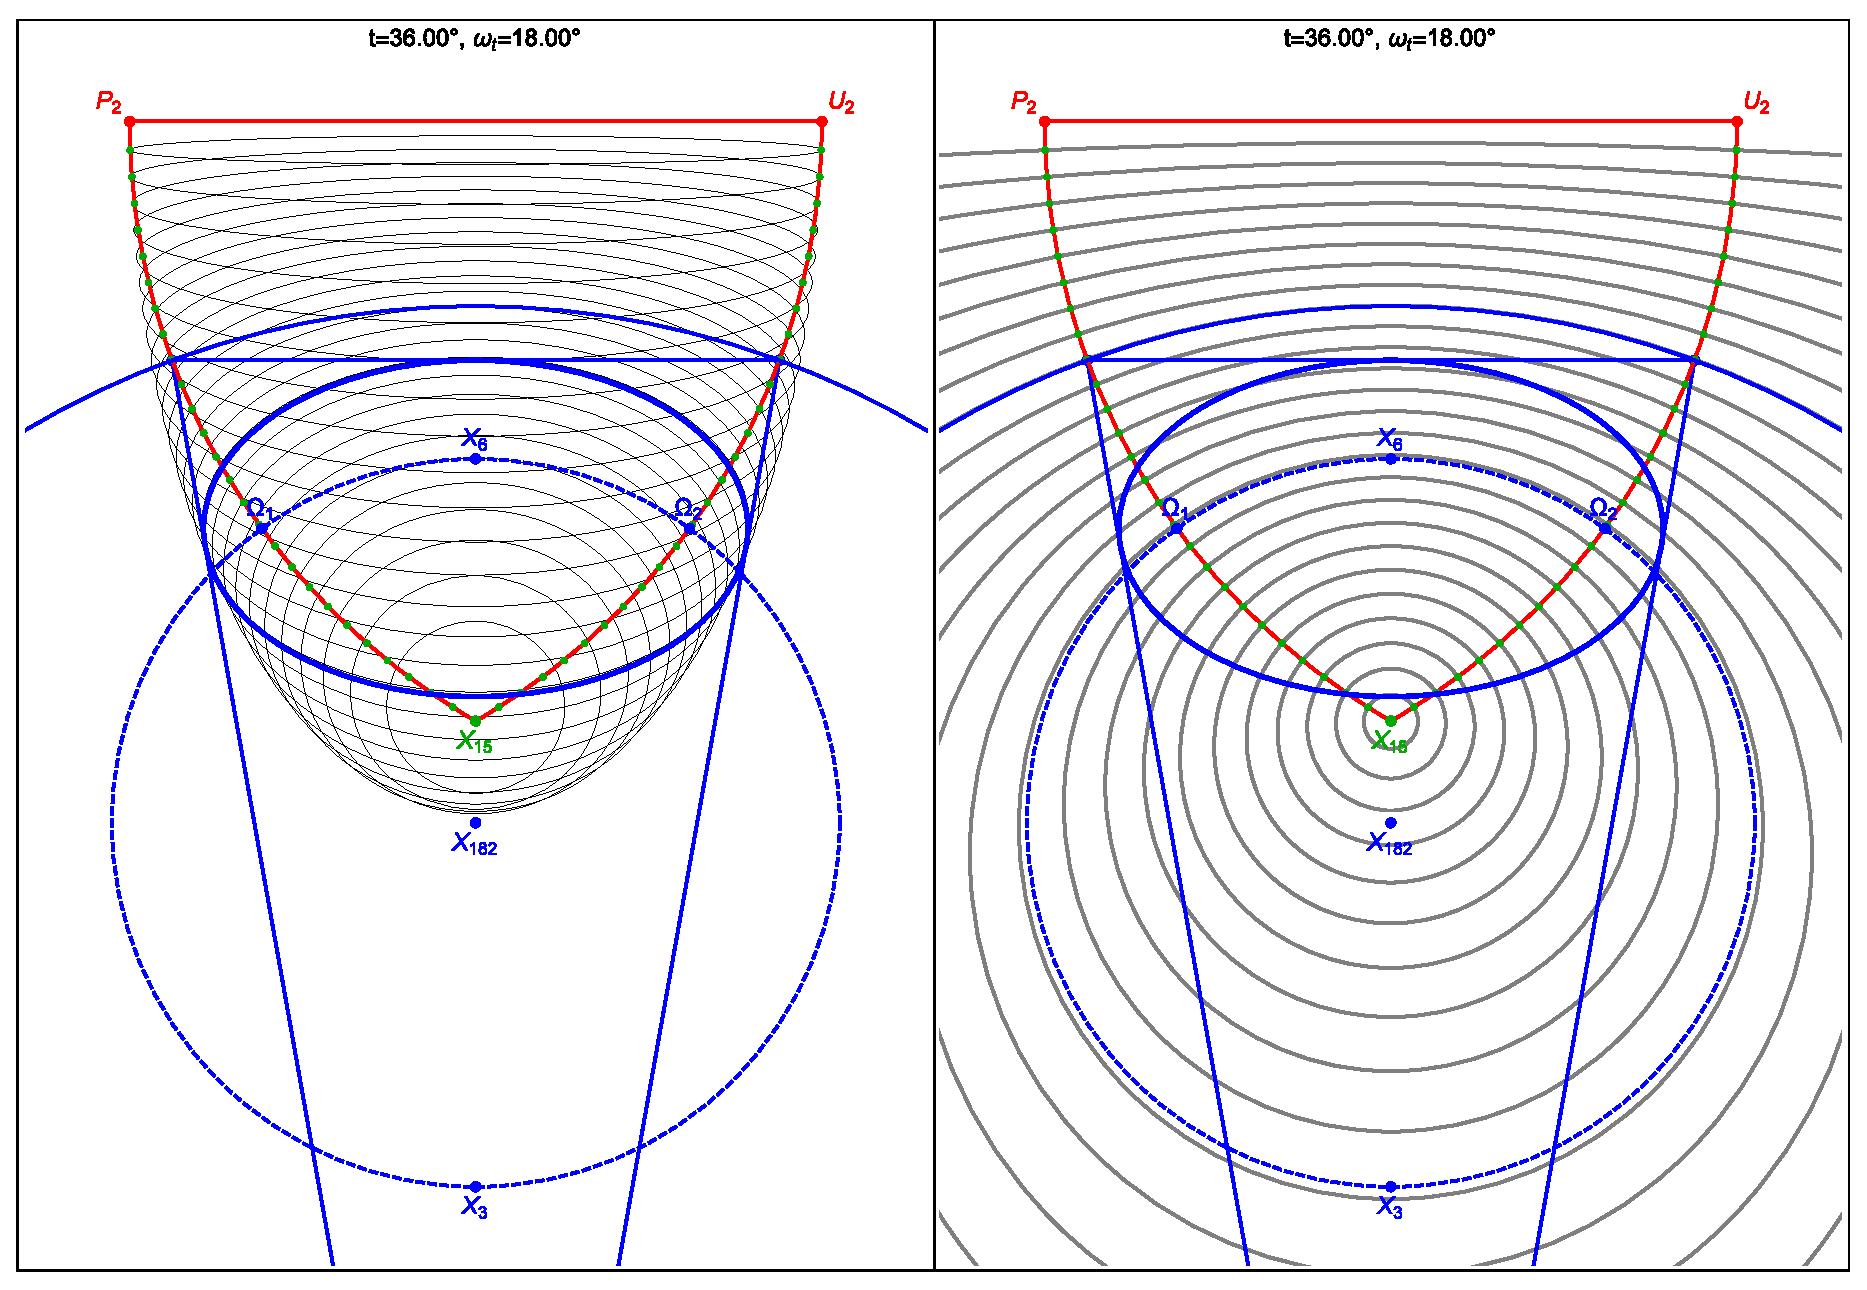
\includegraphics[width=\textwidth]{pics_06_0200_cage_pair.eps}
    \caption{\textbf{Left:} A continuous family of inellipses (gray) is shown with foci (green dots) sliding along two $60^\circ$ circular arcs (red) delimited by $P_2,X_{15}$ and $U_2,X_{15}$. A particular one ($t=36^\circ$) is highlighted (thick blue), with foci $\Omega_1,\Omega_2$. A Brocard porism is formed when $\E_t$ is paired with circle $\Gamma_t$ (blue). An isosceles Poncelet triangle is shown (blue) interscribed in the pair. Also shown is the fixed Brocard circle (dashed blue). \textbf{Right:} The family of circles $\Gamma_t$ (gray) is nested and converges to $X_{15}$. \href{https://youtu.be/jY_8zxBljuk}{Video}}
    \label{fig:cage}
\end{figure}

\begin{proof}
Let $\T$ be the isosceles triangle defined by the vertices $A=f_1$, $B=f_2$ and $C=[0,\frac{\sin t}{2(\cos t  -1)}]$ ($t$ subscripts are omitted). Let vertex $C$ be at the intersection of the line $U_2 f_2$ with the $y$ axis. Applying Lemma \ref{lem:reciprocal} to this triangle it follows that:
\[R'=  \frac {13\,\cos t-3\,\cos 2t -8  }{4 \sin t },\Sha'=\frac {2-\cos t +2}{\sin t} \]

Invert the expressions for $R',\Sha'$ in Theorem \ref{thm:porism} to obtain the anti Brocard triangle $\T^*$ of $\T$, inscribed in $\Gamma_t$. By construction, $C=X_{3}$ of $\T^*$ and the pair $(\E_t,\Gamma_t)$ is a Brocard porism.

%Follows from the relation $[a,b]=  [\frac{R}{\sqrt{1+\Sha^2}}, \frac{2R}{1+\Sha^2}].$
\end{proof}

 %\begin{lemma}
% An  isosceles triangle tangent to $\E_t$ is defined by the vertices
 %\[ A= [ ], B= , C= [0,]
 %\] 
% \end{lemma}

\begin{remark}
Any Brocard porism is a similarity image of a porism $B_t$ defined in Theorem~\ref{thm:continuous_iso}.
\end{remark}

\noindent Referring to Figure~\ref{fig:detach} (right):

\begin{corollary}[Brocard Circle Containment]
Let $s,u\in[0,\pi/3]$ and $s>u$. Then the corresponding Brocard circles $\K_s\subset\K_u$.
\end{corollary}
\begin{proof}
Combining the the expressions for center and radius of $\K_t$ and in Theorem~\ref{thm:continuous_iso} the claim is true if and only if: 
\[\sin(s-u)+\sin u \geq\sin s.\]
\noindent where $s,u\in [0,\frac{\pi}{3}]$ with $s>u$. 
As the above inequation is equivalent to
\[\sin (s-u)(1-\cos u)+\sin u(1-\cos(s-u))\geq 0\] follows the result.
\end{proof}

 \begin{theorem}[Embedding]
 The family of second Brocard triangles of $\B_t$ are Poncelet triangles of a distinct porism $\B_{t'}$, $t'>t$, such that:
 
 \[ \cot{t'}= \Sha' = \frac{4-4\cos{t}+\cos{2t} }{4\sin{t}-\sin{2t}} = \frac{\Sha^2+3}{2\Sha} \]

\label{prop:discrete}
\end{theorem}
 
\begin{proof}
  By Theorem~\ref{thm:continuous_iso}
  the inellipse which yields $\Sha_t$ is given by
    $t=h(\Sha_t)=\tan^{-1}(\frac{2\Sha_t}{\Sha_t^2-1})$.
    From Theorem~\ref{thm:porism} obtain that $\Sha'=g(\Sha_t)=(\Sha_t^2+3)/(2\Sha_t)$. Taking the composition
   $(h\circ g\circ h^{-1})(t)$ leads to the result.
 \end{proof}


\begin{proposition}
 The circles $\K_t$ are perpendicular to $\Cm_1$ and $\Cm_2$
\end{proposition}
\begin{proof} Let 
\begin{align*}
    \Cm_{1,2}:& \;\left(x\pm \frac{1}{2}\right)^2+y^2-1=0\\
    \K_t:&\;x^2+\left(y-\frac{\cos t-2}{2\sin t}\right)^2-\left(\frac{2\cos t-1}{ 2\sin t}\right)^2=0
\end{align*} 

 The intersection of the circles $\Cm_{1,2}$ and $\K_t$
 are the points
 \[
     p_{1,\mp}= \left[  \mp   {\frac {3(2\,\cos t -1)}{2( 5-4\,\cos
t )}},  - {\frac {3\sin t }{ 5-4\,\cos
 t }} \right],\;\;\;
p_{2,\mp}= \left[\mp (\frac{1}{2}-\cos t) , \sin t 
 \right]
\]
Direct calculations show that $\langle \nabla C (p_{i,\mp}),\nabla K(p_{i,\mp})\rangle=0$.
\end{proof}

%\begin{proposition}
% $P_2$ (resp. $U_2$) is the inverse of $\Omega_{1,t}$ (resp. $\Omega_{2,t}$) with respect to $\Gamma_t$. Therefore $P_2,U_2$ are the Beltrami points of each $B_t$, and the triangles $P_2U_2X_{15}$, $P_2U_2X_{16}$ are equilateral.
%\end{proposition}

%\begin{proof}
%It is straightforward to show that the inversion of the foci of $\E_t$ with respect to $\Gamma_t$ as given in Theorem~\ref{thm:continuous} yield $P_2,U_2$ independent of $t$. 
%\end{proof}

\begin{remark}
For any $B_t$, the midpoint  $X_{187}$  of $P_2 U_2$ is the inverse with respect to $\Gamma_t$ of the symmedian point $X_{6,t}$.
\end{remark}

Let $Z_t$ denote the lower vertices of $\E_t$. Setting the derivative of $b$ in Theorem~\ref{thm:continuous_iso} to zero obtain:

\begin{corollary}
 The minor semi-axis $b$ (resp. $Z_t$) of $\E_t$ reverses direction of motion at $t_b=\cos^{-1}(3/4){\simeq}41.41^\circ$ (resp. $t_0=\tan^{-1}(4/3){\simeq}53.13^\circ$). Furthermore $0{\leq}b{\leq}1/4$.
\end{corollary}

Note that the major semi-axis $a$ and the y-coordinate of the upper vertex of $\E_t$ are monotonically decreasing.

\begin{figure}
    \centering
    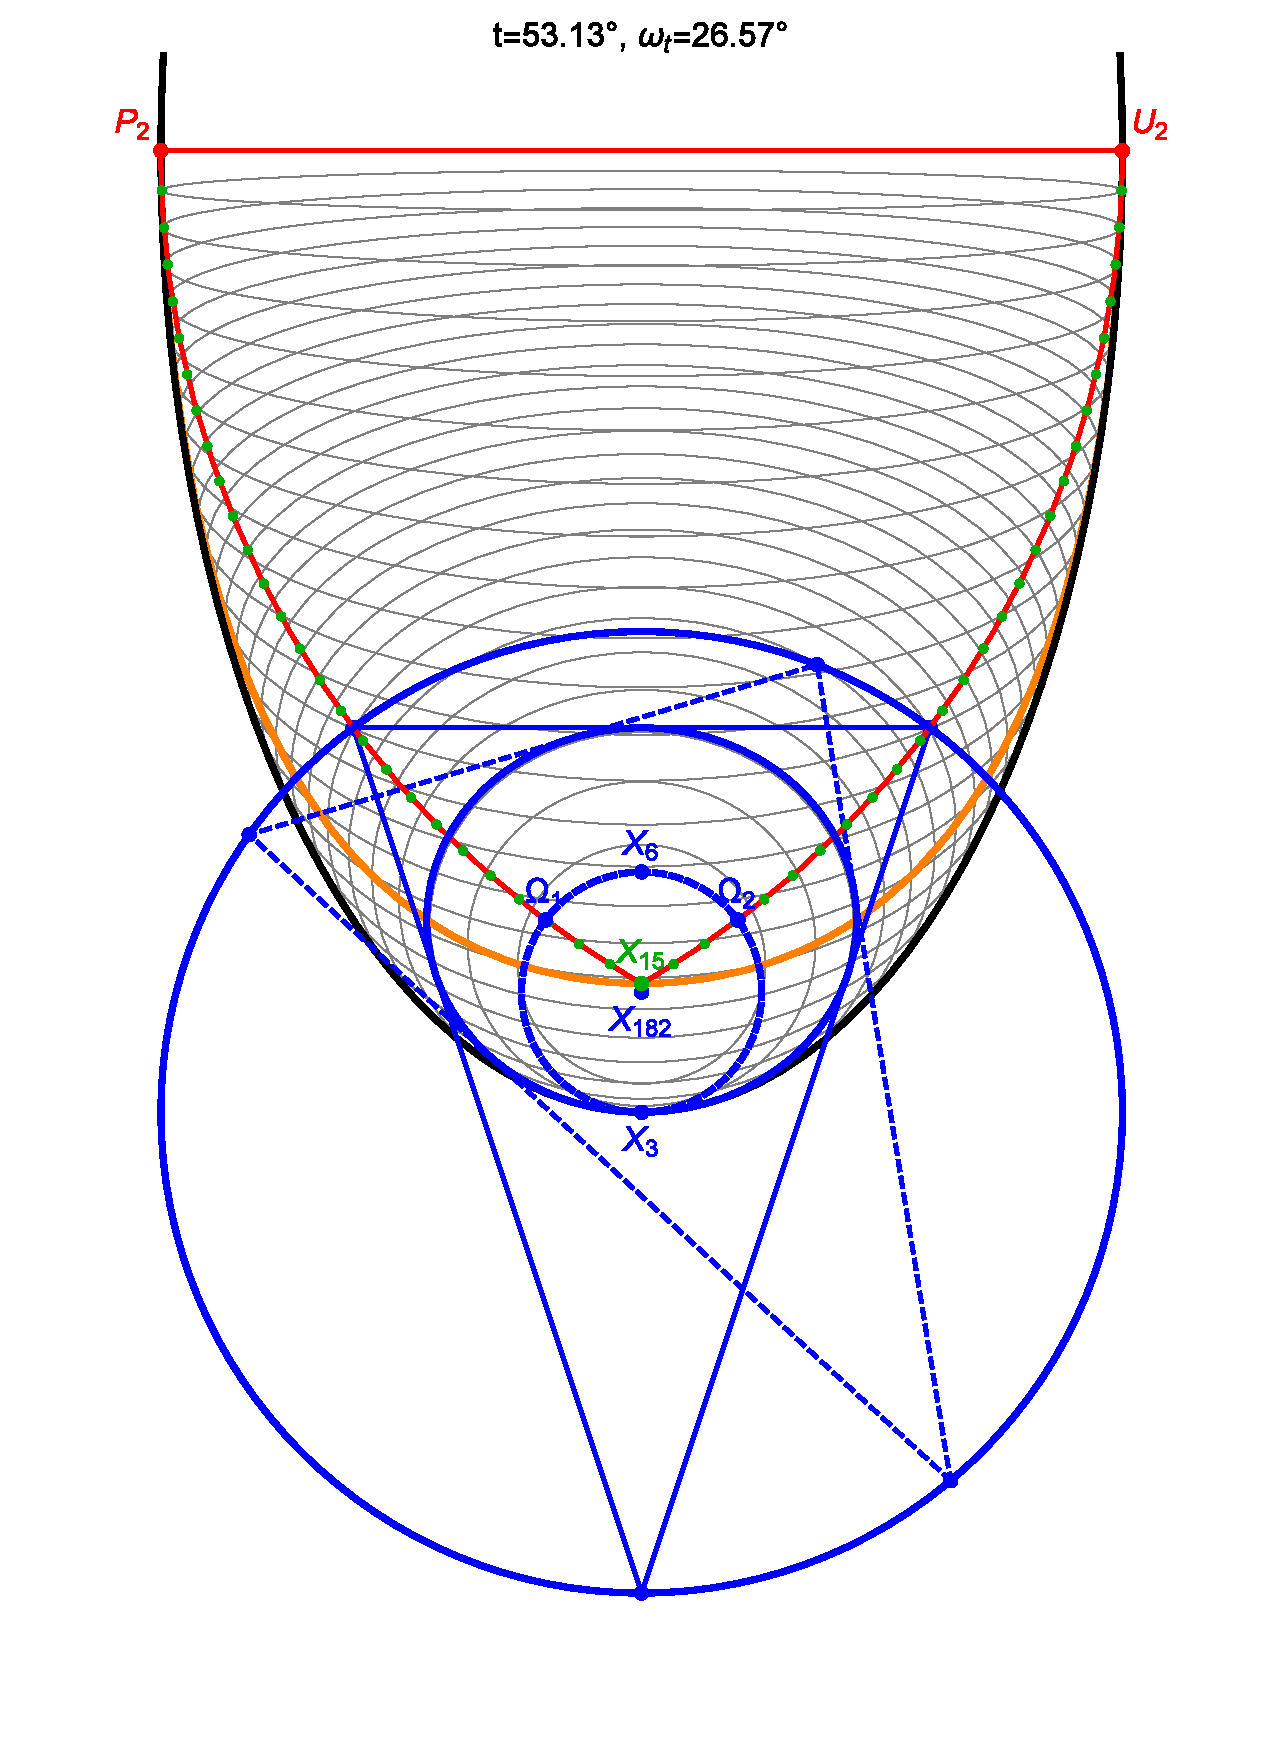
\includegraphics[width=.66\textwidth]{pics_06_0210_detachment.eps}
    \caption{The envelope (thick black) of inellipses $\E_t$ (gray) is an ellipse (only bottom half shown) whose foci are the isodynamic points $X_{15},X_{16}$ common to all families. At $t_0=\cos^{-1}(3/5)$, the porism is such that the Brocard circle (dashed blue) is tangent to $\E_t$ (solid blue), $X_3$ is at the envelope's lower vertex, and the lower vertex of $\E_t$ reverses direction of motion. A non-isosceles Poncelet triangle (dashed blue) is also shown. The locus (orange) of points at which the 3-web formed by the family of inellipses $\E_t$ is perpendicular to the family of Brocard circles $\K_s$ (taken as independent families) is a quartic containing the isodynamic  and Beltrami points; see Remark~\ref{rem:perp-locus}.}
    \label{fig:detach}
\end{figure}

\begin{proposition}
 The envelope $\xi$ of the family $\E_t$ is given by:
 
 \[ \xi_{1,t},\xi_{2,t}= \left[\pm \frac{ \sqrt{5\cos t-3}}{2\sqrt{\cos t+1}},
 -\frac{2\ sin t}{ \cos t+1}
 \right]
 \]
 and this is contained in the ellipse given by
 \[4x^2+y^2-1=0\]
 Furthermore, the isodynamic points $X_{15},X_{16}$ are at its foci.
\end{proposition}

\begin{proof}
 The ellipse $\mathcal{E}_t$ is parametrized by
 \[ \Gamma(u,t)=[a(t)\cos u, b(t)\sin u]+[0,-sin(t)]\]

The envelope is the solution to $\Gamma(u,t)=\Gamma_t(u,t)=0$ which leads to the claim.
\end{proof}

\begin{remark} At $t>t_0=\cos^{-1}(\frac{3}{5})=\tan^{-1}(\frac{4}{3})$ the family $\E_t$ is nested and so the envelope is empty for $t>t_0.$  See Fig. \ref{fig:detach}.
\end{remark}
  
 \begin{proposition}
When $t<\tan^{-1}(\frac{4}{3})$  the Brocard Circle $\K_t$ intersects the Brocard inellipse $\E_t$ at its envelope $\xi_{1,t}$ and $\xi_{2,t}$.
 \end{proposition}
 \begin{proof}
  The Brocard circle passes through the point $[0,-\frac{\sin t}{2(1-\cos t)}  ]$ and it is tangent to the  Brocard inellipse at the point $[0,-1]$ when $\tan{t}=4/3$.
 \end{proof}
 

 
 \begin{proposition}
 The major semi-axis  $a$ is concave and monotonically-decreasing with $a(0)=1, a(\frac{\pi}{3})=0$. The minor semi-axis $b$ is concave with a global maximum $\frac{1}{4}$ attained at $t=\cos^{-1}(\frac{3}{4})$
 and $b(0)=b(\frac{\pi}{3})=0$.
 The eccentricity $\varepsilon(t)=\frac{c(t)}{a(t)} $ is a concave function with $\varepsilon(0)=1, \varepsilon(\frac{\pi}{3})=0$.
 \end{proposition}
 
\begin{proof}
Direct analysis from Theorem \ref{thm:continuous_iso}.
 \end{proof}

Let $V_l(t)\Gamma( -\frac{\pi}{2},t)=[0,-b(t)-\sin{t}]$ denote the lower vertex of $\E_t$.

\begin{corollary}
 $V_l(t)$ moves non-monotonically along the Brocard axis and converges to $X_{15}=[0,-\frac{\sqrt{3}}{2}]$. At $t_0=\tan^{-1}(\frac{4}{5})$ it attains a global minimum $[0,-1]$.
  \label{prop:vertices_ellipse_Et}
\end{corollary}

\begin{proof}  Direct analysis from Theorem~\ref{thm:continuous_iso}.
 \end{proof}

\begin{remark}
 At $t=\tan^{-1}(\frac{4}{5})$,  $\Sha=\frac{5+\sqrt{41}}{4}\approx 2.851$. At $t=\cos^{-1}(\frac{3}{5}) $, $\Sha=2$,
\end{remark}

\begin{remark}
 The family of ellipses $\E_t$ is defined by the implicit differential equation
 \[ 16\,{x}^{2}{y}^{2}\; dx^{2}-8\,xy \left( 4x^2-1 \right){ dx}\,{  dy}+ \left( 16\,{x}^{4}+8\,{x}^{2}+4\,{y}
^{2}-3 \right) dy^{2}=0
 \]
 The family of circles $\K_t$ is given by the differential equation
 \[ 8 x y\; dx-(4x^2-4y^2+3)dy=0\]
 
Consequently, in the interior of the envelope,
the family of circles $\K_t$ and ellipses $\E_t$ define a 3-web \cite{akopyan_2018} which is singular at the coordinate axes and the boundary of the envelope. The orthogonal family to $\K_t$ is the Apollonian
pencil of circles passing through the foci of the envelope. See \cite{akopyan_2018} for the classification of other types of 3-webs defined by circles and ellipses.
\end{remark}
 
\noindent Referring to Figure~\ref{fig:detach}:

\begin{remark}
The families of ellipses $\E_t$ and circles  $\K_s$ (where $t,s$ are independent parameters)
 are orthogonal,
 if and only if,
 \[   16x^4+8x^2+4y^2-3=0.\]
 They are tangent,  if and only if, $x y=0$.
 \label{rem:perp-locus}
 \end{remark}
 
% \begin{proof} The ellipse defined by 
 %\[R=\frac{\sqrt{\Sha^2-3}}{2}, \cos t= %\frac{\Sha^2-1}{\Sha^2+1} \] is similar to $\E_t.$
 %\end{proof}